% Created 2026-04-22 Wed 10:03
% Intended LaTeX compiler: pdflatex
\documentclass[11pt]{article}
\usepackage[utf8]{inputenc}
\usepackage[T1]{fontenc}
\usepackage{graphicx}
\usepackage{longtable}
\usepackage{wrapfig}
\usepackage{rotating}
\usepackage[normalem]{ulem}
\usepackage{amsmath}
\usepackage{amssymb}
\usepackage{capt-of}
\usepackage{hyperref}
\author{Danilo Unapucha, Michael Sornoza, Martin Arevalo, Matías Palomeque}
\date{2026-04-11}
\title{Taller de Configuracion de Entorno WSL}
\hypersetup{
 pdfauthor={Danilo Unapucha, Michael Sornoza, Martin Arevalo, Matías Palomeque},
 pdftitle={Taller de Configuracion de Entorno WSL},
 pdfkeywords={},
 pdfsubject={},
 pdfcreator={Emacs 27.1 (Org mode 9.7.5)}, 
 pdflang={Espanol}}
\begin{document}

\maketitle
\section{Actividades}
\label{sec:orga53eeca}
\subsection{Configuración de WSL con Ubuntu, \LaTeX{}, Python e Emacs}
\label{sec:orgea3eb80}
Danilo Unapucha
\begin{enumerate}
\item Verificación de entorno mamba/anaconda
\begin{verbatim}
     mamba info
\end{verbatim}

\begin{verbatim}

	  libmamba version : 2.5.0
	     mamba version : 2.5.0
	      curl version : libcurl/8.19.0 OpenSSL/3.6.1 zlib/1.3.2 zstd/1.5.7 libssh2/1.11.1 nghttp2/1.68.1 mit-krb5/1.22.2
	libarchive version : libarchive 3.8.6 zlib/1.3.2 liblzma/5.8.2 bz2lib/1.0.8 liblz4/1.10.0 libzstd/1.5.7 liblzo2/2.10 openssl/3.5.5 libb2/bundled
	  envs directories : /home/danilo/miniforge3/envs
	     package cache : /home/danilo/miniforge3/pkgs
			     /home/danilo/.mamba/pkgs
	       environment : base (active)
	      env location : /home/danilo/miniforge3
	 user config files : /home/danilo/.mambarc
    populated config files : /home/danilo/miniforge3/.condarc
	  virtual packages : __unix=0=0
			     __linux=6.6.87=0
			     __glibc=2.39=0
			     __archspec=1=x86_64_v4
		  channels : https://conda.anaconda.org/conda-forge/linux-64
			     https://conda.anaconda.org/conda-forge/noarch
	  base environment : /home/danilo/miniforge3
		  platform : linux-64
\end{verbatim}

\item Verificación de Python
\begin{verbatim}
 python3 --version
\end{verbatim}

\begin{verbatim}
Python 3.13.12
\end{verbatim}

\item Verificación de Emacs
\begin{verbatim}
 emacs --version 
\end{verbatim}

\begin{verbatim}
GNU Emacs 29.3
Copyright (C) 2024 Free Software Foundation, Inc.
GNU Emacs comes with ABSOLUTELY NO WARRANTY.
You may redistribute copies of GNU Emacs
under the terms of the GNU General Public License.
For more information about these matters, see the file named COPYING.
\end{verbatim}

\item Verificación de \LaTeX{}
\begin{verbatim}
 latex --version
\end{verbatim}

\begin{verbatim}
 pdfTeX 3.141592653-2.6-1.40.25 (TeX Live 2023/Debian)
 kpathsea version 6.3.5
 Copyright 2023 Han The Thanh (pdfTeX) et al.
 There is NO warranty.  Redistribution of this software is
 covered by the terms of both the pdfTeX copyright and
 the Lesser GNU General Public License.
 For more information about these matters, see the file
 named COPYING and the pdfTeX source.
 Primary author of pdfTeX: Han The Thanh (pdfTeX) et al.
 Compiled with libpng 1.6.43; using libpng 1.6.43
 Compiled with zlib 1.3; using zlib 1.3
 Compiled with xpdf version 4.04
\end{verbatim}
\end{enumerate}

Sebastian Arevalo
\begin{enumerate}
\item Verificación de entorno mamba/anaconda
\begin{verbatim}
mamba info
\end{verbatim}

\begin{verbatim}

	libmamba version : 2.5.0
	   mamba version : 2.5.0
	    curl version : libcurl/8.19.0 OpenSSL/3.6.1 zlib/1.3.2 zstd/1.5.7 libssh2/1.11.1 nghttp2/1.68.1 mit-krb5/1.22.2
      libarchive version : libarchive 3.8.6 zlib/1.3.2 liblzma/5.8.2 bz2lib/1.0.8 liblz4/1.10.0 libzstd/1.5.7 liblzo2/2.10 openssl/3.5.5 libb2/bundled
	envs directories : /home/danilo/miniforge3/envs
	   package cache : /home/danilo/miniforge3/pkgs
			   /home/danilo/.mamba/pkgs
	     environment : base (active)
	    env location : /home/danilo/miniforge3
       user config files : /home/danilo/.mambarc
  populated config files : /home/danilo/miniforge3/.condarc
	virtual packages : __unix=0=0
			   __linux=6.6.87=0
			   __glibc=2.39=0
			   __archspec=1=x86_64_v4
		channels : https://conda.anaconda.org/conda-forge/linux-64
			   https://conda.anaconda.org/conda-forge/noarch
	base environment : /home/danilo/miniforge3
		platform : linux-64
\end{verbatim}
\item Verificación de Python
\begin{verbatim}
 python --version
\end{verbatim}

\begin{verbatim}
Python 3.13.12
\end{verbatim}
\item Verificación de Emacs
\begin{verbatim}
 emacs --version
\end{verbatim}

\begin{verbatim}
GNU Emacs 29.3
Copyright (C) 2024 Free Software Foundation, Inc.
GNU Emacs comes with ABSOLUTELY NO WARRANTY.
You may redistribute copies of GNU Emacs
under the terms of the GNU General Public License.
For more information about these matters, see the file named COPYING.
\end{verbatim}
\item Verificación de \LaTeX{}
\begin{verbatim}
 latex --version
\end{verbatim}

\begin{verbatim}
 pdfTeX 3.141592653-2.6-1.40.25 (TeX Live 2023/Debian)
 kpathsea version 6.3.5
 Copyright 2023 Han The Thanh (pdfTeX) et al.
 There is NO warranty.  Redistribution of this software is
 covered by the terms of both the pdfTeX copyright and
 the Lesser GNU General Public License.
 For more information about these matters, see the file
 named COPYING and the pdfTeX source.
 Primary author of pdfTeX: Han The Thanh (pdfTeX) et al.
 Compiled with libpng 1.6.43; using libpng 1.6.43
 Compiled with zlib 1.3; using zlib 1.3
 Compiled with xpdf version 4.04
\end{verbatim}
\end{enumerate}

Michael Sornoza
\begin{enumerate}
\item Verificación de entorno mamba/anaconda
\begin{verbatim}
  mamba info
\end{verbatim}

\begin{verbatim}

	 libmamba version : 2.5.0
	    mamba version : 2.5.0
	     curl version : libcurl/8.19.0 OpenSSL/3.6.1 zlib/1.3.2 zstd/1.5.7 libssh2/1.11.1 nghttp2/1.68.1 mit-krb5/1.22.2
       libarchive version : libarchive 3.8.6 zlib/1.3.2 liblzma/5.8.2 bz2lib/1.0.8 liblz4/1.10.0 libzstd/1.5.7 liblzo2/2.10 openssl/3.5.5 libb2/bundled
	 envs directories : /home/danilo/miniforge3/envs
	    package cache : /home/danilo/miniforge3/pkgs
			    /home/danilo/.mamba/pkgs
	      environment : base (active)
	     env location : /home/danilo/miniforge3
	user config files : /home/danilo/.mambarc
   populated config files : /home/danilo/miniforge3/.condarc
	 virtual packages : __unix=0=0
			    __linux=6.6.87=0
			    __glibc=2.39=0
			    __archspec=1=x86_64_v4
		 channels : https://conda.anaconda.org/conda-forge/linux-64
			    https://conda.anaconda.org/conda-forge/noarch
	 base environment : /home/danilo/miniforge3
		 platform : linux-64
\end{verbatim}
\end{enumerate}



\begin{enumerate}
\item Verificación de Python
\begin{verbatim}
 python3 --version
\end{verbatim}

\begin{verbatim}
Python 3.13.12
\end{verbatim}

\item Verificación de Emacs
\begin{verbatim}
 emacs --version
\end{verbatim}

\begin{verbatim}
GNU Emacs 29.3
Copyright (C) 2024 Free Software Foundation, Inc.
GNU Emacs comes with ABSOLUTELY NO WARRANTY.
You may redistribute copies of GNU Emacs
under the terms of the GNU General Public License.
For more information about these matters, see the file named COPYING.
\end{verbatim}

\item Verificación de \LaTeX{}
\begin{verbatim}
 latex --version
\end{verbatim}

\begin{verbatim}
 pdfTeX 3.141592653-2.6-1.40.25 (TeX Live 2023/Debian)
 kpathsea version 6.3.5
 Copyright 2023 Han The Thanh (pdfTeX) et al.
 There is NO warranty.  Redistribution of this software is
 covered by the terms of both the pdfTeX copyright and
 the Lesser GNU General Public License.
 For more information about these matters, see the file
 named COPYING and the pdfTeX source.
 Primary author of pdfTeX: Han The Thanh (pdfTeX) et al.
 Compiled with libpng 1.6.43; using libpng 1.6.43
 Compiled with zlib 1.3; using zlib 1.3
 Compiled with xpdf version 4.04
\end{verbatim}
\end{enumerate}

Matías Palomeque
\begin{enumerate}
\item Verificación de entorno mamba/anaconda
\begin{verbatim}
     mamba info
\end{verbatim}

\begin{verbatim}

	  libmamba version : 2.5.0
	     mamba version : 2.5.0
	      curl version : libcurl/8.19.0 OpenSSL/3.6.1 zlib/1.3.2 zstd/1.5.7 libssh2/1.11.1 nghttp2/1.68.1 mit-krb5/1.22.2
	libarchive version : libarchive 3.8.6 zlib/1.3.2 liblzma/5.8.2 bz2lib/1.0.8 liblz4/1.10.0 libzstd/1.5.7 liblzo2/2.10 openssl/3.5.5 libb2/bundled
	  envs directories : /home/danilo/miniforge3/envs
	     package cache : /home/danilo/miniforge3/pkgs
			     /home/danilo/.mamba/pkgs
	       environment : base (active)
	      env location : /home/danilo/miniforge3
	 user config files : /home/danilo/.mambarc
    populated config files : /home/danilo/miniforge3/.condarc
	  virtual packages : __unix=0=0
			     __linux=6.6.87=0
			     __glibc=2.39=0
			     __archspec=1=x86_64_v4
		  channels : https://conda.anaconda.org/conda-forge/linux-64
			     https://conda.anaconda.org/conda-forge/noarch
	  base environment : /home/danilo/miniforge3
		  platform : linux-64
\end{verbatim}

\item Verificación de Python
\begin{verbatim}
 python3 --version
\end{verbatim}

\begin{verbatim}
Python 3.13.12
\end{verbatim}

\item Verificación de Emacs
\begin{verbatim}
 emacs --version 
\end{verbatim}

\begin{verbatim}
GNU Emacs 29.3
Copyright (C) 2024 Free Software Foundation, Inc.
GNU Emacs comes with ABSOLUTELY NO WARRANTY.
You may redistribute copies of GNU Emacs
under the terms of the GNU General Public License.
For more information about these matters, see the file named COPYING.
\end{verbatim}

\item Verificación de \LaTeX{}
\begin{verbatim}
 latex --version
\end{verbatim}

\begin{verbatim}
 pdfTeX 3.141592653-2.6-1.40.25 (TeX Live 2023/Debian)
 kpathsea version 6.3.5
 Copyright 2023 Han The Thanh (pdfTeX) et al.
 There is NO warranty.  Redistribution of this software is
 covered by the terms of both the pdfTeX copyright and
 the Lesser GNU General Public License.
 For more information about these matters, see the file
 named COPYING and the pdfTeX source.
 Primary author of pdfTeX: Han The Thanh (pdfTeX) et al.
 Compiled with libpng 1.6.43; using libpng 1.6.43
 Compiled with zlib 1.3; using zlib 1.3
 Compiled with xpdf version 4.04
\end{verbatim}
\end{enumerate}

\subsection{Comandos emacs tutorial}
\label{sec:org5b925f7}
Danilo Unapucha
\begin{center}
\begin{tabular}{llll}
Comando & Descripción & Comando & Descripción\\[0pt]
\hline
C-l & Me ayuda a ver de mejor manera el texto ya que me lo pone arriba o en la mitad o abajo & C-k & Ayuda mucho al poder eliminar toda la linea en la que me encuentro\\[0pt]
M-k & Este elimina toda una oración y ayuda bastante al eliminar todo un párrafo si no se esta conforme & C-g & Este es el mas importante ya que cierra el minibuffer o el comando para sacarnos de un apuro\\[0pt]
\end{tabular}
\end{center}

Sebastian Arevalo
\begin{center}
\begin{tabular}{llll}
Comando & Descripción & Comando & Descripción\\[0pt]
\hline
C-d & Sirve para suprimir un carácter en el que estoy trabajando muy útil en refacción. & M-w & Permite tener la función de copiar texto seleccionado\\[0pt]
C-a & Es bastante útil a la hora de programar de manera en la que no debes buscar el inicio de linea & C-y & Ayuda muchísimo al dar la función de pegar texto copiado\\[0pt]
\end{tabular}
\end{center}

Michael Sornoza

\begin{center}
\begin{tabular}{llll}
Comando & Descripción & Comando & Descripción\\[0pt]
\hline
C-<SPACE> & Me ayuda a seleccionar texto & M-< & Te regresa al principio del documento es como la tecla inicio\\[0pt]
C-x C-f & Permite abrir un archivo & C-x b & Cambiar entre buffers\\[0pt]
\end{tabular}
\end{center}

Matias Palomeque
\begin{center}
\begin{tabular}{llll}
Comando & Descripción & Comando & Descripción\\[0pt]
\hline
C-n & Avanza una línea. Permite buscar información de manera rápida & C-v & Avanza una página. Permite leer un texto de manera más rápida\\[0pt]
M-e & Mueve al cursor al inicio de la siguiente oración & C-u & Permite darle un parámetro numérico a ciertos comandos.\\[0pt]
\end{tabular}
\end{center}


\subsection{Comandos Emacs Juego}
\label{sec:org87a5460}
Danilo Unapucha
\begin{center}
\begin{tabular}{rr}
Iteración & Puntaje\\[0pt]
\hline
1 & 140\\[0pt]
2 & 140\\[0pt]
3 & 140\\[0pt]
\end{tabular}
\end{center}
\begin{enumerate}
\item Iteración 1
\begin{center}
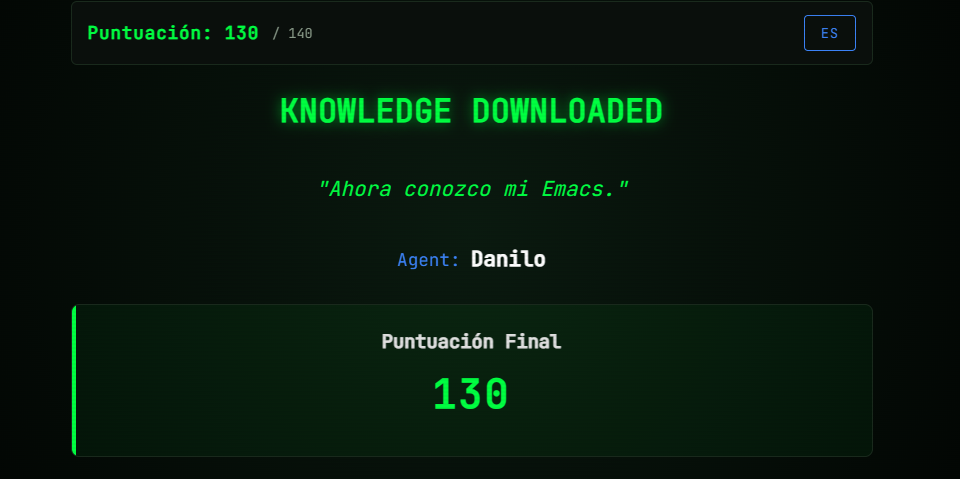
\includegraphics[width=.9\linewidth]{./images/juego1.png}
\end{center}
\item Iteración 2
\begin{center}
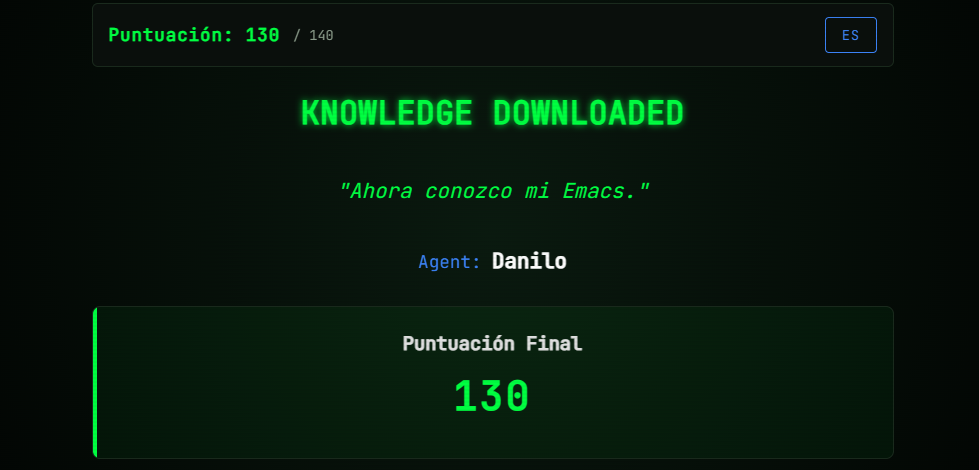
\includegraphics[width=.9\linewidth]{./images/juego2.png}
\end{center}
\item Iteración 3
\begin{center}
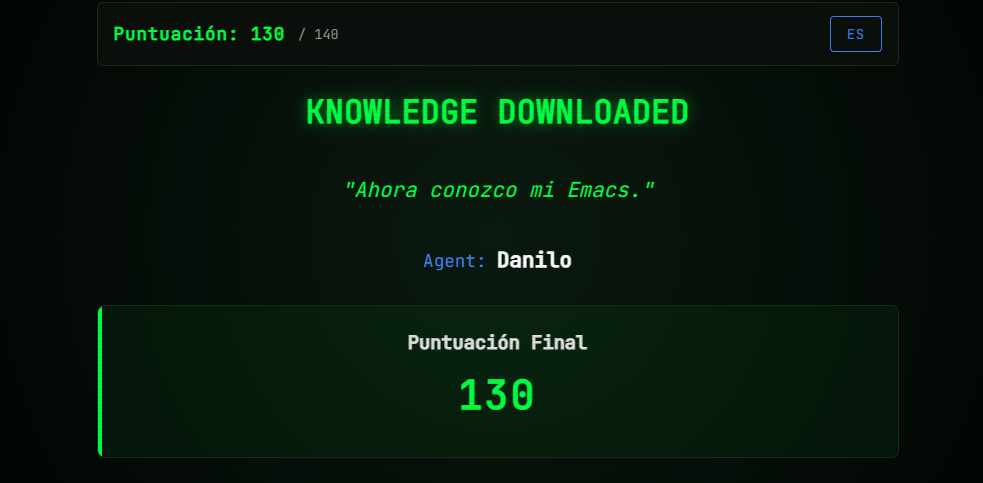
\includegraphics[width=.9\linewidth]{./images/juego3.png}
\end{center}
\end{enumerate}

Sebastian Arevalo
\begin{center}
\begin{tabular}{rr}
Iteración & Puntaje\\[0pt]
\hline
1 & 130\\[0pt]
2 & 130\\[0pt]
3 & 125\\[0pt]
\end{tabular}
\end{center}
\begin{enumerate}
\item Iteración 1
\begin{center}
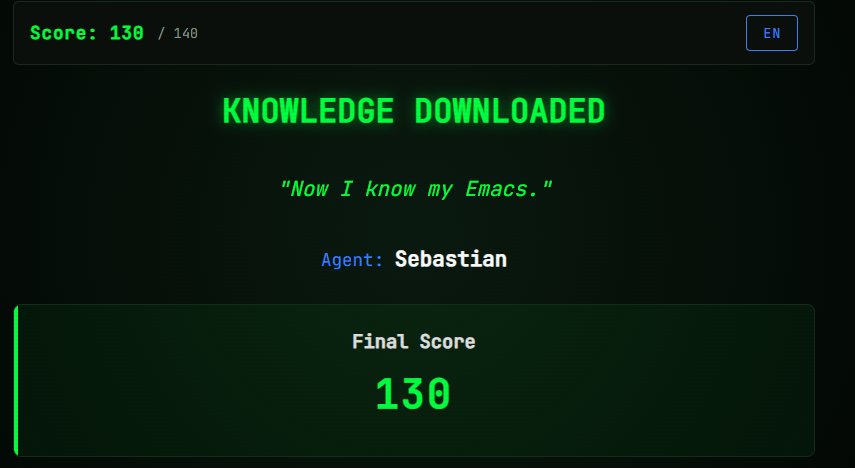
\includegraphics[width=.9\linewidth]{./images/Juego1_Sebas.png}
\end{center}
\item Iteración 2
\begin{center}
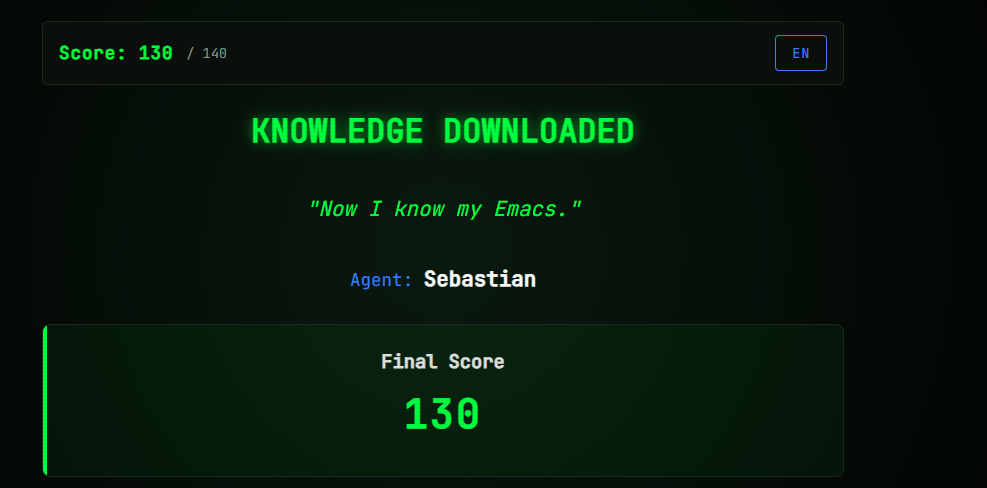
\includegraphics[width=.9\linewidth]{./images/Juego2_Sebas.png}
\end{center}
\item Iteración 3
\begin{center}
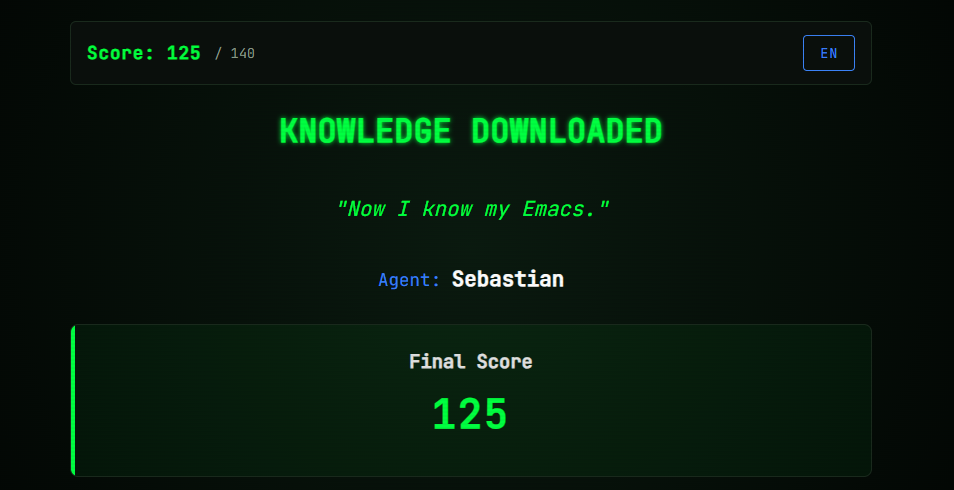
\includegraphics[width=.9\linewidth]{./images/Juego3_Sebas.png}
\end{center}
\end{enumerate}


Michael Sornoza
\begin{center}
\begin{tabular}{rr}
Iteración & Puntaje\\[0pt]
\hline
1 & 122\\[0pt]
2 & 140\\[0pt]
3 & 140\\[0pt]
\end{tabular}
\end{center}

\begin{enumerate}
\item Iteración 1
\begin{center}
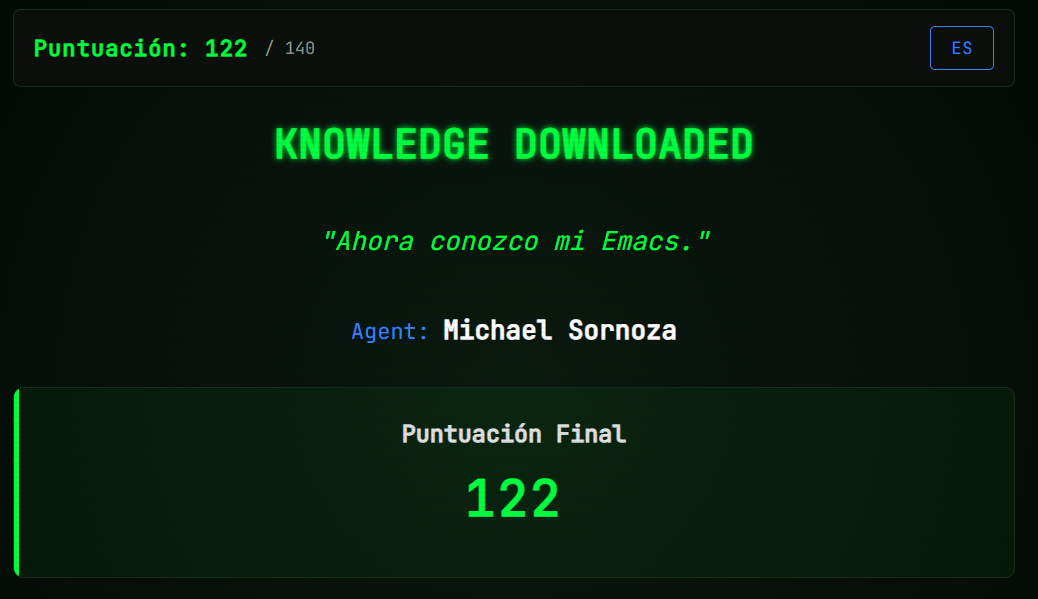
\includegraphics[width=.9\linewidth]{./images/juego1_michael.png}
\end{center}
\item Iteración 2
\begin{center}
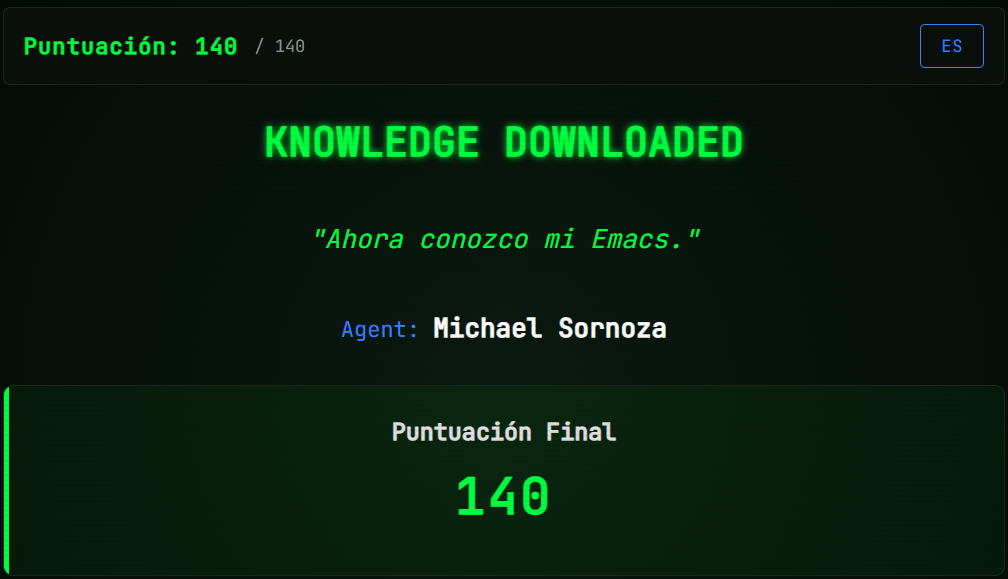
\includegraphics[width=.9\linewidth]{./images/juego2_michael.png}
\end{center}
\item Iteración
\begin{center}
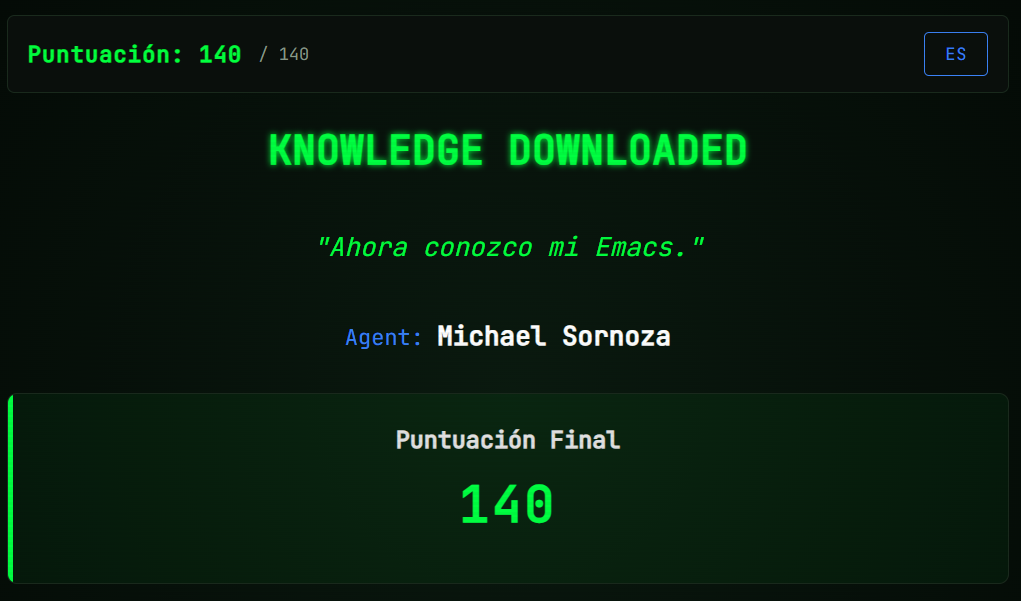
\includegraphics[width=.9\linewidth]{./images/juego3_michael.png}
\end{center}
\end{enumerate}

Matías Palomeque
\begin{center}
\begin{tabular}{rr}
Iteración & Puntaje\\[0pt]
\hline
1 & 128\\[0pt]
2 & 128\\[0pt]
3 & 140\\[0pt]
\end{tabular}
\end{center}

\begin{enumerate}
\item Iteración 1
\begin{center}
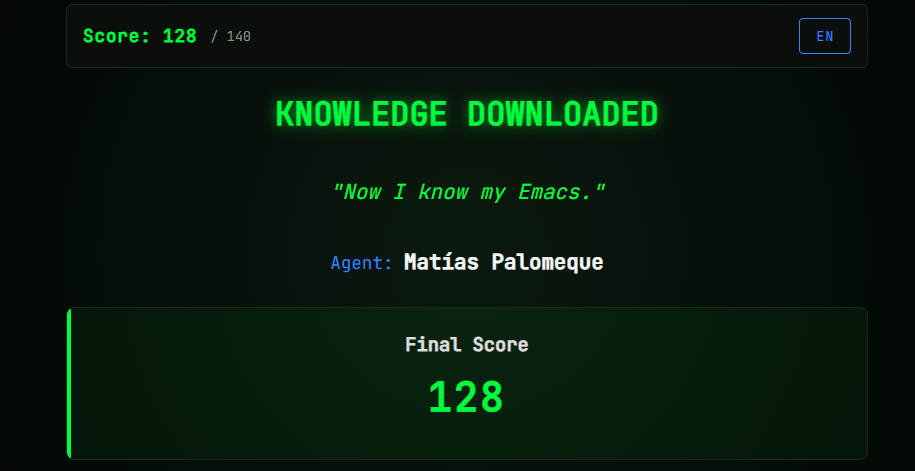
\includegraphics[width=.9\linewidth]{./images/juego10.png}
\end{center}
\item Iteración 2
\begin{center}
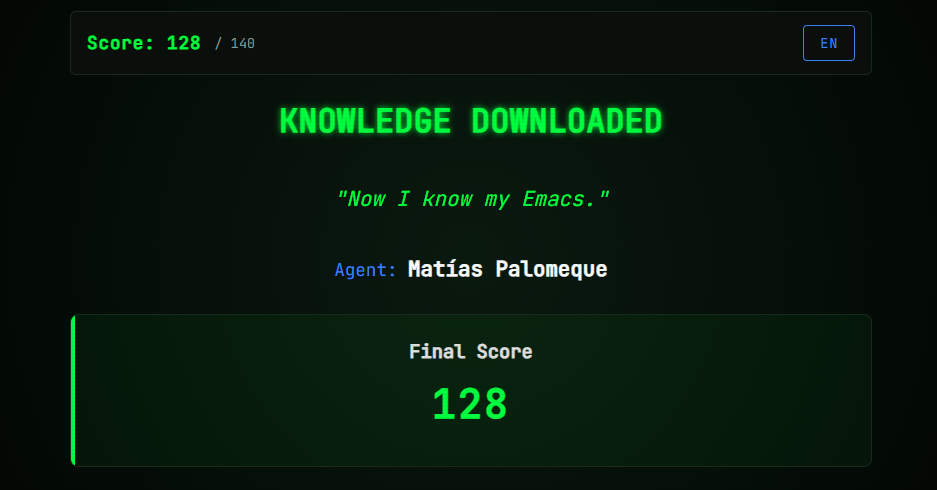
\includegraphics[width=.9\linewidth]{./images/juego11.png}
\end{center}
\item Iteración 3
\begin{center}
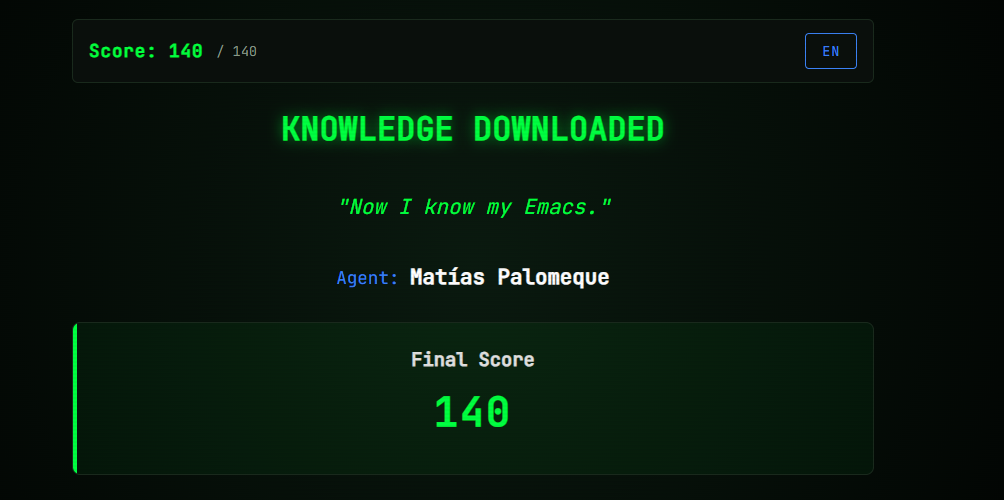
\includegraphics[width=.9\linewidth]{./images/juego12.png}
\end{center}
\end{enumerate}


\subsection{Usando Emacs para tener Ayuda sobre Emacs}
\label{sec:org708b40a}
\textbf{\textbf{Comandos Fáciles}}
\begin{enumerate}
\item \textbf{\textbf{Danilo Unapucha}} C-n. Move cursor vertically down ARG lines.
\item \textbf{\textbf{Sebastian Arevalo}} C-x C-s Save currend buffer
\item \textbf{\textbf{Michael Sornoza}} C-a. Runs the command org-beginning-of-line (found in org-mode-map).
\item \textbf{\textbf{Matias Palomeque}} M-f. Move point forward ARG words (backward if ARG is negative).
\end{enumerate}

\textbf{\textbf{Comandos Dificiles}}
\begin{enumerate}
\item \textbf{\textbf{Danilo Unapucha}} C-v. Scroll text of selected window upward ARG lines; or near full screen if no ARG.
\item \textbf{\textbf{Sebastian Arevalo}} C-k kill or remove de line where the cursor is at.
\item \textbf{\textbf{Michael Sornoza}} C-u Runs the command universal-argument (found in global-map), which is an interactive native-compiled Lisp function in ‘simple.el’.
\item \textbf{\textbf{Matias Palomeque}} C-/. Undo some previous changes.
\end{enumerate}
\subsection{Equipo de Trabajo}
\label{sec:org2274a0b}
\begin{center}
\begin{tabular}{lll}
Nombre & email & Rol\\[0pt]
\hline
Danilo Unapucha & danilo.unapucha@epn.edu.ec & Lider\\[0pt]
 &  & \\[0pt]
 &  & \\[0pt]
Matías Palomeque & matias.palomeque@epn.edu.ec & Colaborador\\[0pt]
 &  & \\[0pt]
 &  & \\[0pt]
Sebastian Arevalo & martin.arevalo@epn.edu.ec & Colaborador\\[0pt]
 &  & \\[0pt]
 &  & \\[0pt]
Michael Sornoza & michael.sornoza@epn.edu.ec & Colaborador\\[0pt]
\end{tabular}
\end{center}


\subsection{Verificación de Entregables}
\label{sec:orge592dc4}
\begin{itemize}
\item[{$\boxtimes$}] Verificación de configuración de entorno WSL y paquetes del curso.
\item[{$\boxtimes$}] Tutorial de Comandos Emacs realizado.
\item[{$\boxtimes$}] Captura de Imágenes y puntajes de Emacs Trainer App.
\item[{$\boxtimes$}] Usando Emacs para tener ayuda sobre Emacs
\item[{$\boxtimes$}] Verifique que estén los nombres de los integrantes del equipo e identificado el líder.
\item[{$\boxtimes$}] Revisión de ortografía con ispell en el buffer
\item[{$\boxtimes$}] Generación de Archivo PDF M-x org-latex-export-to-pdf
\end{itemize}
\end{document}
